%!TEX root = labo.tex

\chapter{Introduction to the Internet Lab}

What you will learn in this lab:
\begin{itemize}
	\item Overview of the equipment
	\item Saving your data
	\item Navigating your way around Linux
	\item Working with protocol analysers: \cmd{tcpdump}, Wireshark
\end{itemize}

\newpage
\setsession{prelab1}
\section{Prelab 1}\label{sec:prelab1}
%!TEX root = labo.tex
\subsection*{Basic Linux commands}
Before entering the lab, you should familiarise yourself with some basic Linux commands and the Wireshark network analyser tool.

\subsubsection*{Man Pages}
The PCs run the Linux operating system, a Unix-like operating system. This assignment asks you to review some Unix commands. Man pages exist on every lab machine. You can also find the manual pages (``man pages'') online at

\qquad \url{http://manpages.ubuntu.com/}

For each of the following commands, type the name of the command as a search term. The search will return the appropriate man page.

Read the man pages of the following commands for the operating system version ``\osversion'':

\qquad \cmd{man}, \cmd{pwd}, \cmd{ls}, \cmd{more}, \cmd{mv}, \cmd{cp}, \cmd{rm}, \cmd{mkdir}, \cmd{rmdir}, \cmd{chmod}, \cmd{kill}, \cmd{ping}, \cmd{tcpdump}

\subsubsection*{Wireshark}
The man page for Wireshark, a network analyser tool, can be found on every lab machine. You can also read about the Wireshark network analyzer at the website
\url{https://www.wireshark.org/docs/}.
Read the introduction and the manual pages of Wireshark.

\newpage
\subsection*{Prelab Questions}

\begin{questions}
	\q{1}{What will happen if you type \cmd{man man} in Linux?}
	\q{2}{How can you use the command \cmd{ls} to find out about the size of file \path{/etc/fstab}?}
	\q{3}{What happens if you have two files with names \path{file1} and \path{file2} and you type \cmd{mv file1 file2}? Which option of \cmd{mv} issues a warning in this situation?}
	\q{4}{What is the command that you issue if you are in directory \path{/} and want to copy the file \path{/mydata} to directory \path{/labdata}?}
	\q{5}{What is the command that you issue if you are in directory \path{/} and want to copy all files and directories under directory \path{/mydirectory} to directory \path{/newdirectory}?}
	\q{6}{What happens if you type the command \cmd{rm *} in a directory?}
	\q{7}{What is the command that you issue if you want to delete all files and directories under the directory \path{/mydirectory}?}
\end{questions}


\newpage
\setsession{lab1}
\section{Lab 1}\label{sec:lab1}

In Lab 1, you will acquaint yourself with the equipment of the Internet Lab, the Linux operating system, and some traffic measurement tools.

\newpage
\subsection{Getting Started}
\subsubsection*{Lab reservations}

You need to book labs in advance at: \url{https://student.mosaic.uantwerpen.be/telecomlabo/}. To be able to go online you need to register and accept the terms of service published here: \url{https://euterpe.mosaic.uantwerpen.be/laboaccess/}.

\subsubsection*{Cables}

When you have booked a lab, you can ask for a box of cables in room M.G.236 (go through the server room M.G.235). The box contains a set of UTP cables in different colors and 1 cross-cable. Please return it when you are done.

\newpage
\subsection{Overview of the Internet Lab Hardware}

Each lab is equipped with:
\begin{itemize}
	\item 4 PC's, each equipped with their own monitor, keyboard, mouse and external USB hub. 
	\item 4 10BASE-T Hubs
	\item 1 10BASE-T/100BASE-TX Hub
	\item Patch panel: The interfaces of each of the PC's are connected with a patch panel, which means that it should not be necessary to change any of the network cabling directly on the PC.
	\item 4 Cisco 1760 routers.
\end{itemize}

\subsubsection*{Using the lab PC's for Computer Networks Lab}

It is important to know that on booting the PC's all previous changes are automatically flushed from the system, returning them to their original state.

\emph{Note: Please contact one of the course instructors to recover any lost files if the PC was accidentally shut down.}

You need to log in using your UA credentials. Make sure yo select the ``telecomlabo'' option in the login screen! This will disable all network related services on the device and configure the network stack for the Lab. Not doing this might affect your lab results.

When working in the terminal either use \cmd{sudo} before each command to get root privileges.

\begin{cmdblock}
	> sudo ip addr add 192.168.1.2/24 dev eth0
\end{cmdblock}

Or type in \cmd{sudo su -} at the beginning of each new terminal session to keep working with root privileges.

\begin{cmdblock}
	> sudo su -
\end{cmdblock}

You will be asked for a password when using the \cmd{sudo} command. For the remainder of this course, whenever a password is requested that is not your own student password, you should use \cmd{mvkbj1n}, which is derived from the phrase "Met veel kabels bouw je één netwerk".

Please turn off the lab PC's and screens when you are done with them.

\subsubsection*{Setting up an uplink to the internet}

Each lab PC should have 3 interfaces (\iface{eth0}, \iface{eth1} and \iface{internet}). \iface{eth0} and \iface{eth1} are meant for your lab setups, while the latter interface can be used to set up an uplink to the Internet. There is an icon ``Enable Internet Access'' on the desktop, double-click it and follow the instructions. You will be asked to enter you UA credentials. 

\emph{Note: to go online you will have to first register at: \url{http://euterpe.mosaic.uantwerpen.be/laboaccess}}

\subsubsection*{Removing the uplink to the internet}

When performing any of the lab tests it is recommended that they are not connected to the internet. This makes sure that the configurations made for the Internet uplink do not interfere with the lab setup. To remove the uplink double-click on the icon 'Disable Internet Access' on the desktop.

\newpage
\subsection{Saving files}

Each PC is configured with a USB hub that is placed next to the monitor. You can connect a USB stick to the computer and copy your results and traces to it. You can either do this using the file manager or from the command line. The USB sticks are automatically mounted in the \path{/media/} directory.

Make sure to unmount your stick before removing to avoid any data loss, either via the icon on the destop or on the command line using the \cmd{umount} command.

\begin{cmdblock}
	umount /media/usbstick/
\end{cmdblock}

We would like to stress again that, on booting the PC's, all previous changes are automatically flushed from the system, returning them to their original state.

You can use the simple single segment network that we will be discussing in Part 4 to copy files from one computer to another over the network. You can use tools like \cmd{scp} or \cmd{rsync} to do this. Please check the man pages of the programs on how to use them.

If Internet access is working you can also copy your files to an external server:

\begin{cmdblock}
	> scp -r /root/lab1/ user@student.mosaic.uantwerpen.be:labocomputernetwerken/
\end{cmdblock}

The above example will copy all files and directories from the \path{/root/lab1/} directory to the \path{labocomputernetwerken} directory in the user's home folder on student.mosaic.uantwerpen.be.

\newpage
\subsection{Setting up your first network}

We will now construct the simple single segment network shown in Figure \ref{fig:lab1-network} that we will be using throughout the remainder of this lab.

\begin{figure}[ht]
	\centering
	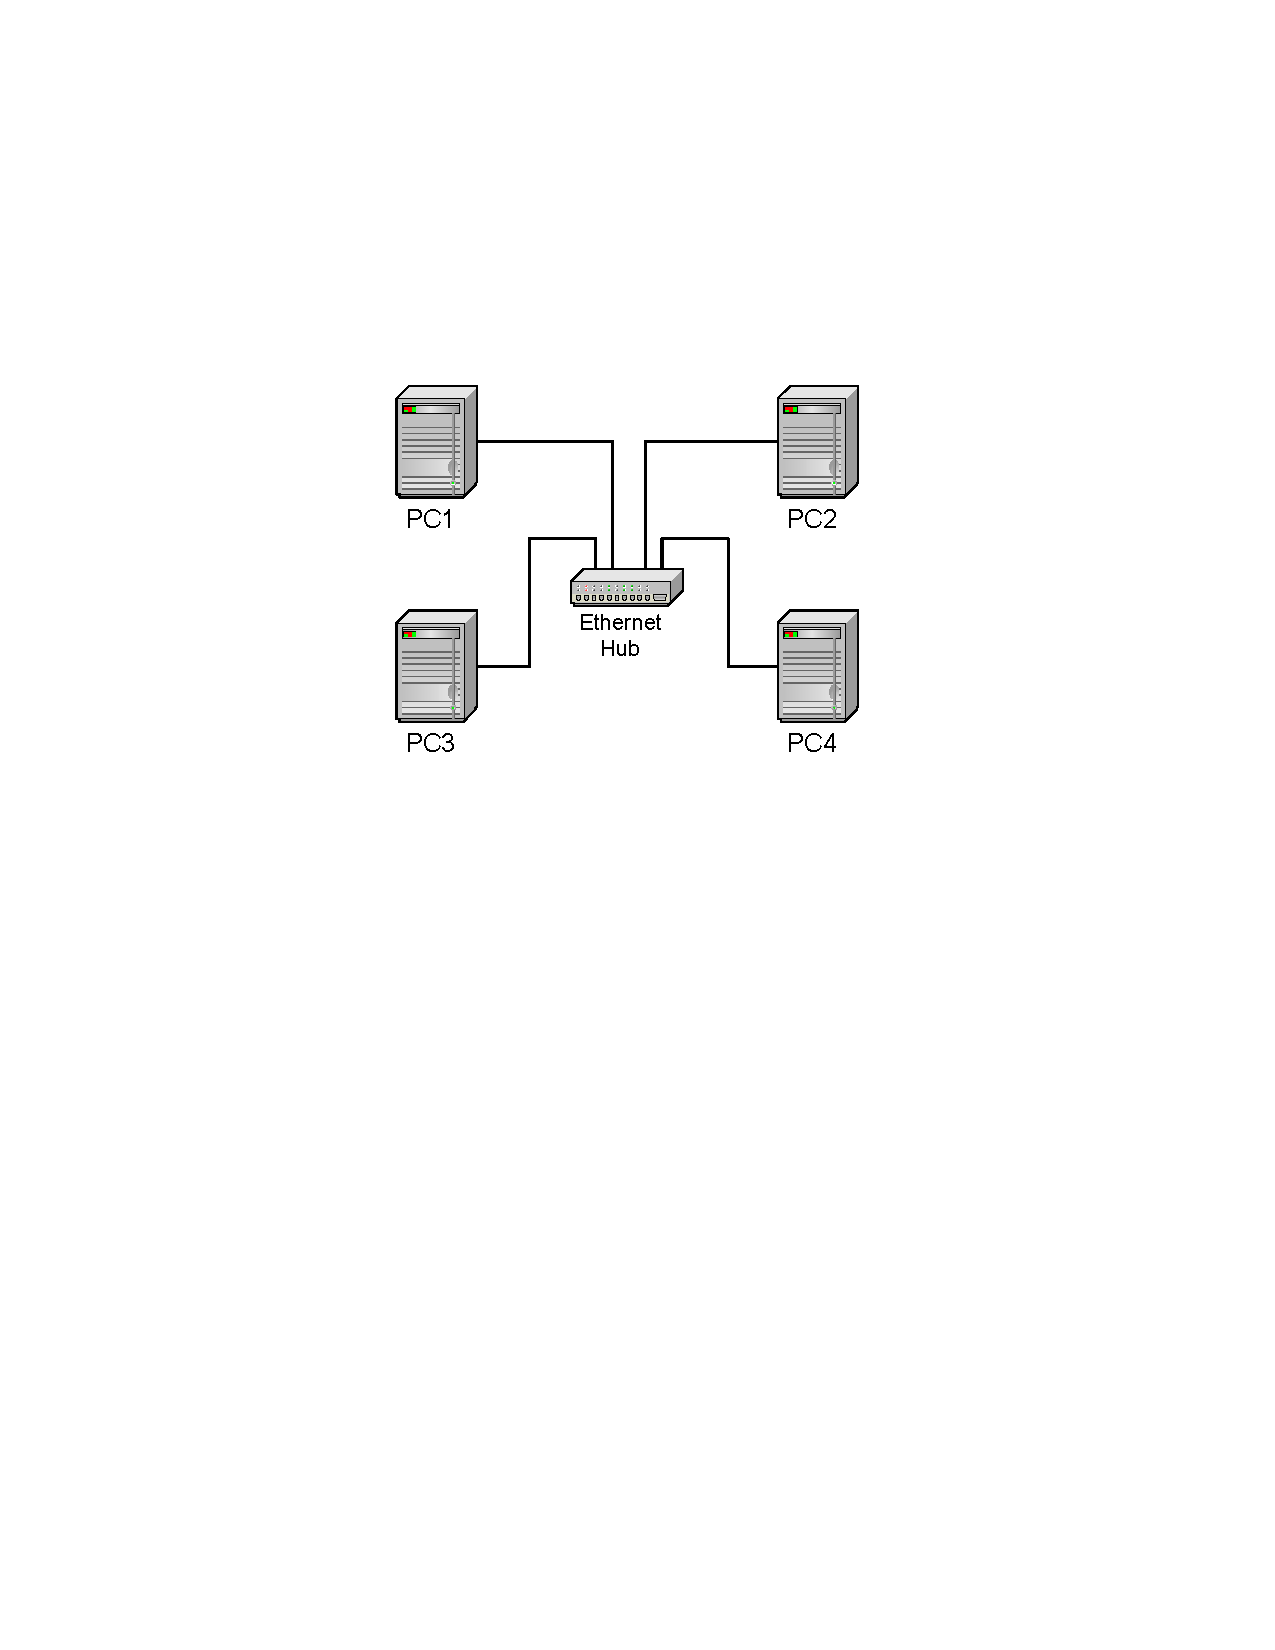
\includegraphics{graphics/lab1-network.pdf}	
	\caption{Network configuration for Lab 1.}
	\label{fig:lab1-network}
\end{figure}

\begin{itemize}
	\item All four Linux PCs are connected to a single Ethernet segment via a single hub as shown in Figure \ref{fig:lab1-network}.
	\item IP addresses for the Linux PCs are configured as in Table \ref{tab:lab1-ip-addresses}
		\begin{table}[ht]
			\centering
			\begin{tabular}{| c | c | c |}	
				\hline
				\textbf{Linux PC} & \textbf{IP Addresses of Ethernet Interface \iface{eth0}}  \\ \hline
				PC1 & 10.0.1.11/24 \\ 
				PC2 & 10.0.1.12/24 \\
				PC3 & 10.0.1.13/24 \\
				PC3 & 10.0.1.14/24 \\ \hline
			\end{tabular}
			\caption{IPv4 addresses for Lab 1}
			\label{tab:lab1-ip-addresses}
		\end{table}
	\item The notation 10.0.1.11/24 means that the IP address is 10.0.1.11 and the network prefix is 24 bits long. A network prefix of 24 bits corresponds to a netmask set to 255.255.255.0. With this netmask, all hosts are on the 10.0.1.0/24 network.
\end{itemize}


\subsubsection*{Mapping of the patch panel ports to the PC interfaces}
\begin{enumerate}
	\item Use the mapping in Table \ref{tab:lab1-patch-panel} to figure out which interface of which PC is which port on the patch panel. Connect the PC's to the hub using Ethernet cables.
		\begin{table}[ht]
			\centering
			\begin{tabular}{| c | c | c |}	
				\hline
				\textbf{Linux PC} & \textbf{Interface} & \textbf{Patch panel port}  \\ \hline
				PC1 & \iface{eth0} & 1 \\ 
				PC1 & \iface{eth1} & 2 \\ 
				PC2 & \iface{eth0} & 3 \\ 
				PC2 & \iface{eth1} & 4 \\ 
				PC3 & \iface{eth0} & 5 \\ 
				PC3 & \iface{eth1} & 6 \\ 
				PC4 & \iface{eth0} & 7 \\ 
				PC4 & \iface{eth1} & 8 \\ \hline
			\end{tabular}
			\caption{IP addresses for Lab 1}
			\label{tab:lab1-patch-panel}
		\end{table}
	\item Configure \iface{eth0} for each of the PCs. e.g. for PC1 use the following command.
		\begin{cmdblock}
	PC1% ifconfig eth0 10.0.1.11 netmask 255.255.255.0 broadcast 10.0.1.255 up
		\end{cmdblock}
		As an alternative, you can use th \cmd{ip} command:
		\begin{cmdblock}
	PC1% ip addr add 10.0.1.11/24 dev eth0
	PC1% ip link set dev eth0 up
		\end{cmdblock}
	\item Test connectivity by using \cmd{ping}, e.g.
		\begin{cmdblock}
	PC1% ping -c 5 10.0.1.11
		\end{cmdblock}
	\end{enumerate}

\newpage
\subsection{Locating Configuration Files in Linux}

Linux has numerous configuration files which set the environment variables of the operating system. For example, if you want to set up your Linux PC as an IP router, you merely need to change a single line in one of the configuration files. Studying configuration files also provides a way of learning what network configuration options are available to you.

\remark If you are unable to revert some of the changes you made, try rebooting the PC's as they will be reverted to their original settings.

\remark Configuration files are fundamentally different across different versions of Unix-like operating system (e.g., AIX, Solaris, Linux, FreeBSD). Sometimes the structure of configuration files changes between releases of the same Unix version. For example, the configuration files of different Linux distributions, such as, Ubuntu, Fedora, OpenSuSE at and Slackware, are quite different. Furthermore, the configuration files between different versions of the same Linux distribution can have significant differences.

The file \path{/etc/network/interfaces} contains settings on how the interfaces should be configured when starting the network service on Debian-based Linux distributions. You will notice that there is not much in this file as our lab PCs are preconfigured NOT to bring up their interfaces. You can read the man page to find out more on this file. It will not be used in the remainder of this course.

\begin{cmdblock}
	> man interfaces
\end{cmdblock}

You will not find much in \path{sysctl.conf} either: check out the \cmd{sysctl} tool and briefly browse \path{/proc/sys/net}. You will see that there are several parameters that allow you to tweak the behavior of the linux network stack.

\begin{cmdblock}
	> ls /proc/sys/net
	> man sysctl
\end{cmdblock}

The \path{/etc/hosts} files contains a mapping of hostnames to IP addresses.

\begin{cmdblock}
	> less /etc/hosts
\end{cmdblock}

\subsubsection*{Exercise 5. Network configuration files}
\begin{questions}
	\q{5.1}{Which file(s) must be edited to change the name of a Linux PC (e.g. from PC1 to machine1)?}
	\q{5.2}{Which file(s) include information that determines whether a Linux PC performs IP forwarding?}

\end{questions}

\newpage
\subsection{Using Ping}

One of the most basic, but also most effective tools to debug IP networks is the \cmd{ping} command. The ping command tests whether another host or router on the Internet is reachable. The \cmd{ping} command sends an ICMP Echo Request datagram to an interface, and expects an ICMP Echo Reply datagram in return.

Note:
\begin{itemize}
	\item On Linux systems, \cmd{ping} continues to send packets until you interrupt the command with the \cmd{Ctrl-c} keys.
	\item When using \cmd{ping} on the Linux PCs, we recommend to always send at least two ICMP Echo Request packets. We have observed that in some occasions, the first ICMP Echo Request may be dropped at the receiver.
\end{itemize}

\subsubsection*{Exercise 6. Issuing ping commands}

\begin{enumerate}
	\item From PC1, send 5 ping messages (using the -c option) to PC2. Save the output. 
		\begin{cmdblock}
	PC1% ping -c 5 10.0.1.12
		\end{cmdblock}
	\item On PC2, issue a ping to the IP address of PC1. Also, issue a \cmd{ping} command to the \iface{loopback} interface, \cmd{127.0.0.1}. Limit the number of pings to 5. Save the output.
\end{enumerate}

\begin{questions}
	\q{6.1}{Include the output you saved in the exercise.}
	\q{6.2}{Explain the difference between pinging the local Ethernet interface and the \iface{loopback} interface. Specifically, on PC1, what is the difference between typing \cmd{ping 10.0.1.11} and \cmd{ping 127.0.0.1}? (This is a conceptual question on the role of the \iface{loopback} interface. The response to the ping command does not provide you with the answer to this question.) Hint: Try using \cmd{tcpdump} or Wireshark, which are explained in the next section to verify your answer. Hint: Is this handled by software (the linux routing stack), hardware (the network card, hubs, switches, routers) or both?}
	\q{6.3}{Find a host connected to the Internet. Send ping messages to a number of web servers on the Internet and collect statistics on the maximum round-trip delay of the ICMP Echo Request/Echo Reply. Try to find a host with a very long round-trip time. To avoid overloading the destination, do not send more than 10 ping packets to any destination machine. Save the output data and include it in your lab report.}
\end{questions}

\newpage
\subsection{Basics of \cmd{tcpdump}}

\cmd{tcpdump} allows you to capture traffic on a network and display the packet headers of the captured traffic. \cmd{tcpdump} can be used to identify network problems or to monitor network activities.

\subsubsection*{Exercise 7-A. Simple \cmd{tcpdump} exercise}

Use \cmd{tcpdump} to observe the network traffic that is generated by issuing \cmd{ping} commands.
\begin{framed}
	If you use the \cmd{tee} or \cmd{tail} commands to simultaneously view and save the output from \cmd{tcpdump}, you need to use the \cmd{-l} option of \cmd{tcpdump}. For example:
	\begin{cmdblock}
	> tcpdump -n -l > filename & tail -f filename
	> tcpdump -n -l | tee filename
	\end{cmdblock}
	\emph{Note: It may be necessary to hit \cmd{Ctrl-c} to terminate the \cmd{tcpdump} session. In some situations, it may be best to simply redirect the output of \cmd{tcpdump} straight to a file (e.g., \cmd{tcpdump \textgreater filename}) and view it afterwards with the \cmd{less} command or a text editor.}
\end{framed}

\begin{enumerate}
	\item Switch to PC1. Start \cmd{tcpdump} so that it monitors all packets that contain the IP address of PC2, by typing
		\begin{cmdblock}
	PC1% tcpdump -n host 10.0.1.12
		\end{cmdblock}
	\item Open a new window and execute
		\begin{cmdblock}
	PC1% ping -c 1 10.0.1.12
		\end{cmdblock}
	\item Observe the output of \cmd{tcpdump}. Save the output to a file.
\end{enumerate}

\begin{questions}
	\q{7.A}{Include the saved output in your lab report. Explain the meaning of each field in the captured data.}
\end{questions}

\subsubsection*{Exercise 7-B. Another \cmd{tcpdump} traffic capture}
\begin{enumerate}
	\item On PC1, start capturing packets using the \cmd{tcpdump -n} command.
	\item Issue a ping to the non-existing IP address 111.111.111.111:
		\begin{cmdblock}
	PC1% ping -c 1 111.111.111.111
		\end{cmdblock}
	\item Issue a ping to the broadcast address 10.0.1.255 using the command:
		\begin{cmdblock}
	PC1% ping -c 2 -b 10.0.1.255
		\end{cmdblock}
		When sending pings to the broadcast address is not working, check out the \path{/proc/sys/net/ipv4/} directory for possible broadcast-related settings. Try enabling/disabling them if necessary (see the previous paragraph).
		\boxinfo{Explain what you did, what happened and why in the lab report. Simply stating that broadcast pings didn't work is not a correct answer.}
	\item Save the outputs of \cmd{ping} and \cmd{tcpdump} to a file.
\end{enumerate}

\begin{questions}
	\q{7.B}{Include the saved output in your lab report and interpret the results. How many of the Linux PCs responded to the broadcast ping? Why is this?}
\end{questions}

\newpage
\subsection{Basics of wireshark}

Wireshark is a network protocol analyzer with a graphical user interface. Using Wireshark, you can interactively capture and examine network traffic, view summaries and get detailed information for each packet.

\subsubsection*{Exercise 8. Running wireshark}

This exercise walks you through the steps of capturing and saving network traffic with Wireshark. The exercise is conducted on PC1.

\begin{figure}[ht]
	\centering
	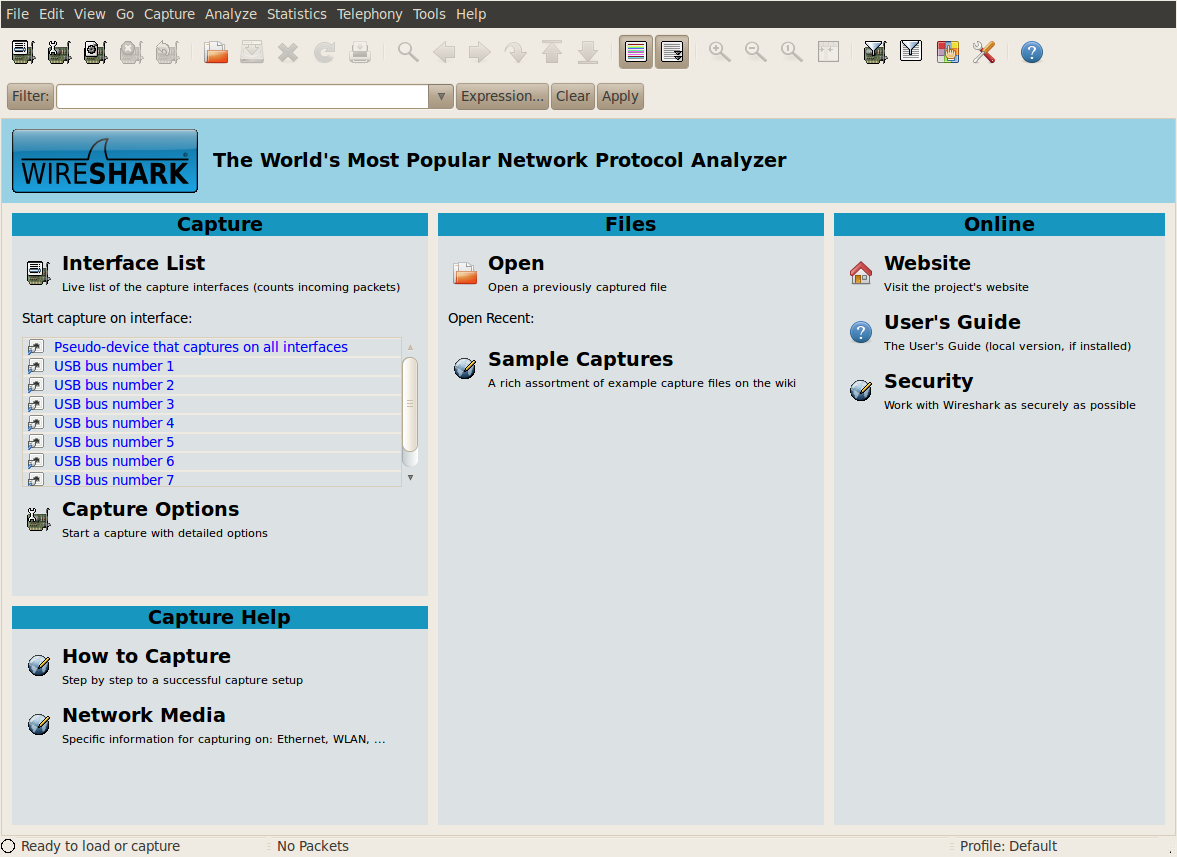
\includegraphics[width=\linewidth]{graphics/wireshark-main-updated.png}	
	\caption{Wireshark Main Window.}
	\label{fig:lab1-wireshark-main}
\end{figure}

\begin{enumerate}
	\item Starting Wireshark: On PC1, start Wireshark by typing 
		\begin{cmdblock}
	PC1% wireshark
		\end{cmdblock}
		This displays the Wireshark main window on your desktop as shown in Figure \ref{fig:lab1-wireshark-main}.
		\boxwarning{\textbf{Do not forget to start Wireshark with root permissions using \cmd{sudo} if you are not root already.}}
	\item Selecting the capture options: Use the instructions in Figure \ref{fig:lab1-capture-options} to set the options of Wireshark in preparation for capturing traffic. Use the same options in other labs, whenever Wireshark is started.
		\par
		\begin{minipage}{\linewidth}
			\begin{framed}
				\centering
				\textbf{Selecting capture preferences in Wireshark}
				\begin{enumerate}
					\item From the main window, select ``Capture:Start''.
					\item This displays the following ``Capture Preferences'' window:\par
						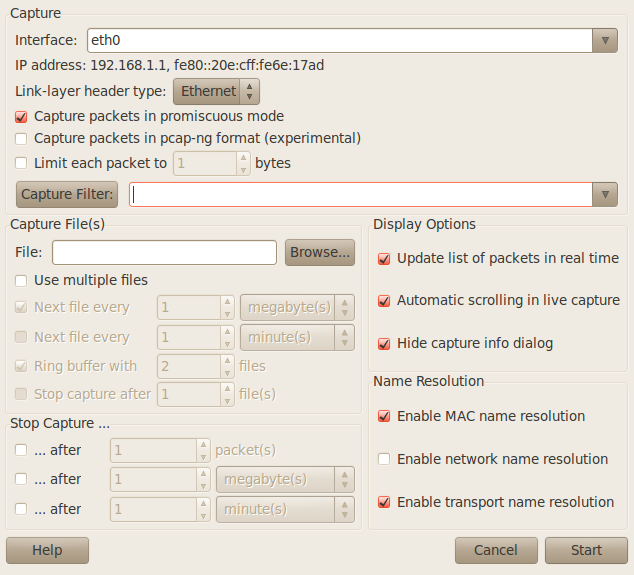
\includegraphics[width=\linewidth]{graphics/capture-options-updated.png}
						\begin{itemize}
							\item Select \iface{eth0} in ``Interface''.
							\item Select ``Capture packets in promiscuous mode''.
							\item Select ``Update list of packets in real time''.
							\item Select ``Automatic scrolling in live capture''.
							\item Unselect ``Enable MAC name resolution''.
							\item Unselect ``Enable network name resolution''.
							\item Unselect ``Enable transport name resolution''.
						\end{itemize}
				\end{enumerate}
			\end{framed}
			\captionof{figure}{General capture settings for Wireshark}
			\label{fig:lab1-capture-options}
		\end{minipage}

	\item Starting the traffic capture: Start the packet capture by clicking ``OK'' in the ``Capture Preferences'' window.

	\item Generating traffic: In a separate window on PC1, execute a \cmd{ping} command to PC3.
		\begin{cmdblock}
	PC1% ping -c 2 10.0.1.13
		\end{cmdblock}
		Observe the output in Wireshark's main window.
		Click and highlight a captured packet in the Wireshark window, and view the headers of the captured traffic.

	\item Stopping the traffic capture: Click ``Stop'' in the window ``Ethernet Capture''.

	\item Saving captured traffic: Save the results of the captured traffic as a plain text file. Use the instructions in Figure \ref{fig:lab1-print-options} in order to configure the print options..\par
		\begin{minipage}{\linewidth}
			\begin{framed}
				\centering
				\textbf{Selecting print options for saving captured traffic to plain text files}
				\begin{enumerate}
					\item From the main window, select ``File:Print''.
					\item This displays the following ``Printer oprions'' window:\par
					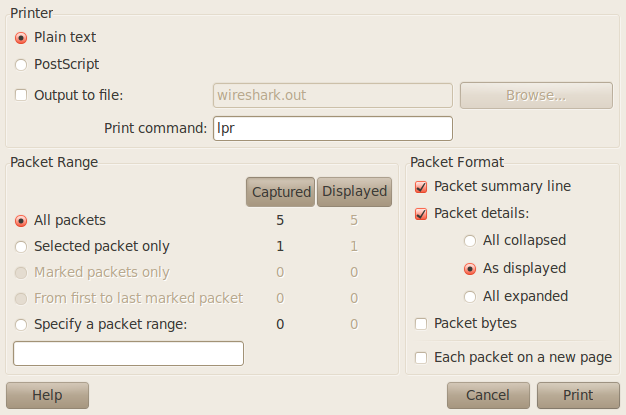
\includegraphics[width=\linewidth]{graphics/wireshark-print-updated.png}
					\begin{itemize}
						\item Select the format ``PlainText''.
						\item Select the ``File'' checkbox and type the filename in the field next to the ``File'' button.
						\item Select ``Print summary'' if you want to save only some high level information on each packet. Print summary is usually sufficient.
						\item Select ``Print detail'' and ``Expand all levels'' if you want to save all details of all packets at all levels.
						\item Click the ``OK'' button to complete the save operation.
					\end{itemize}
				\end{enumerate}
			\end{framed}
			\captionof{figure}{Selecting print options.}
			\label{fig:lab1-print-options}
		\end{minipage}\hspace*{\fill}
			\boxinfo{If you select ``Save'' in the ``File'' menu, the captured data is saved in the format of a libpcap file. This format can be interpreted by both \cmd{tcpdump} and Wireshark. Measurements saved in libpcap format can be analyzed at a later time. However, libpcap files are not plain text files and are not useful for preparing your report.}
			\boxinfo{In general, unless asked to do otherwise, always select the ``Print summary'' option when you include saved data in the lab report. This will help keep the length of the lab report reasonably small. If detailed information is required you will be asked to save ``details'' of the captured traffic. In this case, select the ``Print detail'' option.}
			\boxwarning{\textbf{Always include binary libpcap traces with your report, in addition to printed summaries or details that you use in the report to prove your answer is correct.}}
\end{enumerate}

\begin{questions}
	\q{8}{Include the file with the captured data in your lab report. Save the details of the captured traffic using the ``Print Detail'' option in the ``Print'' Window. Describe the differences between the files saved by \cmd{tcpdump} (in Part 7) and by Wireshark (in this part).}
\end{questions}
